\documentclass[10pt,twocolumn]{article}

\usepackage[T1]{fontenc}
\usepackage{lmodern}
\usepackage{microtype}
\usepackage[a4paper,top=18mm,bottom=20mm,left=17mm,right=17mm,columnsep=7mm]{geometry}
\usepackage{amsmath,amssymb,amsthm,mathtools,bm}
\usepackage{booktabs,tabularx,array}
\usepackage{graphicx}
\usepackage{tikz}
\usetikzlibrary{arrows.meta,positioning,calc}
\usepackage{xcolor}
\usepackage{url}
\usepackage{placeins}
\usepackage{hyperref}
\usepackage[nameinlink,capitalise]{cleveref}
\usepackage{authblk}
\usepackage{balance}

\definecolor{linkblue}{HTML}{174A7E}
\definecolor{darkgreen}{HTML}{246B45}
\hypersetup{
  colorlinks=true,
  linkcolor=linkblue,
  citecolor=darkgreen,
  urlcolor=linkblue,
  pdftitle={Temporal Order Changes a Bounded-Memory Information-Recovery Frontier},
  pdfauthor={Javier Emilio Baz\'an S\'anchez},
  pdfsubject={Causal list decoding and rank-tail bounds for streaming quantum memory},
  pdfkeywords={quantum memory, temporal order, quantum combs, entanglement fidelity, list decoding}
}

\graphicspath{{../figures/}}
\setlength{\emergencystretch}{2em}
\setlength{\parindent}{1em}
\setlength{\parskip}{0pt}
\raggedbottom
\renewcommand{\topfraction}{0.95}
\renewcommand{\dbltopfraction}{0.95}
\renewcommand{\textfraction}{0.04}
\renewcommand{\floatpagefraction}{0.78}
\renewcommand{\dblfloatpagefraction}{0.78}

\newtheorem{theorem}{Theorem}[section]
\newtheorem{lemma}[theorem]{Lemma}
\newtheorem{proposition}[theorem]{Proposition}
\newtheorem{corollary}[theorem]{Corollary}
\theoremstyle{remark}
\newtheorem{remark}[theorem]{Remark}

\newcommand{\Tr}{\operatorname{Tr}}
\newcommand{\id}{\mathbb I}
\newcommand{\ket}[1]{\lvert #1\rangle}
\newcommand{\bra}[1]{\langle #1\rvert}
\newcommand{\proj}[1]{\lvert #1\rangle\!\langle #1\rvert}
\newcommand{\PA}{P_{\mathrm A}}
\newcommand{\FR}{F_{\mathrm R}}
\newcommand{\BG}{B_{4,2}}
\newcommand{\UI}{U_{\mathrm I}}
\newcolumntype{Y}{>{\raggedright\arraybackslash}X}

\newenvironment{resultbox}
  {\par\smallskip\noindent\begin{minipage}{\columnwidth}\small
   \color{linkblue}\rule{\columnwidth}{0.5pt}\par\smallskip
   \textbf{Main consequence.}\enspace\color{black}}
  {\par\smallskip\color{linkblue}\rule{\columnwidth}{0.5pt}\end{minipage}\par\smallskip}

\title{{\normalsize\color{linkblue}\bfseries CARMEN-Q}\\[0.25em]
\textbf{Temporal Order Changes a Bounded-Memory\\Information--Recovery Frontier}\\
\large Causal list decoding and a linear rank-tail theorem}
\author[1]{Javier Emilio Baz\'an S\'anchez}
\affil[1]{Facultad de Ciencias, Universidad Nacional Aut\'onoma de M\'exico, Mexico City, Mexico\\
\texttt{bazan@ciencias.unam.mx}}
\date{22 August 2026}

\begin{document}
\maketitle

\begin{abstract}
Can the temporal order of the same linear predicate change the operational
power of a fixed quantum memory? A verifier streams four halves of independent
EPR pairs through a device, sequestering each output before the next input.
Only after commitment does a late choice request either the complete two-bit
syndrome (AUDIT) or coherent recovery of all four pairs (RETURN). The device
has one persistent qubit and unlimited genuinely classical transcript. Two
check matrices contain the same columns: the grouped order
$(e_1,e_1,e_2,e_2)$ and the interleaved order
$(e_1,e_2,e_1,e_2)$. The grouped order attains the full static qubit frontier
and permits return fidelity $1/2$ at perfect audit. The interleaved order is
instead bounded by, and attains, $1/4$. More generally, $m$ consecutive
full-rank syndrome blocks impose a temporal product law at perfect audit.
The main result makes that law robust: if $D$ is the input dimension and
$\epsilon=1-\PA$, the spectral mass below the perfect-audit rank is at most
$mD\epsilon$. Causal dimension-to-list conversion, Schur--Horn majorisation,
and flagged polar recovery then give an explicit approximate-audit bound. For
the interleaved instance this certifies a strict order-dependent support gap
for every $3/7<\lambda<1$, including balanced weight. A local
Pauli-completion theorem also reduces the arbitrary adaptive optimum exactly
to one normalised bond-two Choi MPS. A compact three-effect MPS reaches
$0.759802783851\ldots$ at balanced weight and agrees with unrestricted
variational searches, but the global maximum of the nonconvex MPS quotient
remains uncertified.
\end{abstract}

\noindent\textbf{Keywords:} bounded coherent memory; temporal order; quantum
combs; entanglement recovery; syndrome decoding; Ky Fan norms.

\section{Introduction}

Memory dimension is a natural resource in a multitime quantum process, but
dimension alone does not say how difficult a temporal task is. A memory may
need to preserve several partial functions simultaneously, and the number of
live functions can change when otherwise identical inputs are reordered. This
work isolates that phenomenon in a late-choice information--recovery game.

The verifier sends fresh entangled carriers one at a time. A device must commit
each output before seeing the next input and does not learn the terminal task
in advance. AUDIT rewards a classical syndrome of the stream, whereas RETURN
rewards preservation of the unknown quantum inputs. A coherent memory can
accumulate a syndrome reversibly; a classical record that helps AUDIT also
damages RETURN. The question is whether a mere permutation of the syndrome
columns changes the best tradeoff when the coherent memory is fixed.

It does. The pair in \cref{fig:orders} uses the same rank-two binary code and
the same one-qubit memory. Grouping equal columns realizes the complete static
qubit frontier. Interleaving them creates two consecutive full-rank temporal
blocks and lowers perfect-AUDIT return fidelity from $1/2$ to $1/4$. The
effect is not limited to an endpoint: a robust rank-tail theorem proves a
strict support-function separation throughout $3/7<\lambda<1$.

The remaining interior optimisation can be stated without an unbounded
adaptive tree. Every normalised bond-two Choi leaf admits a local
four-outcome Pauli completion whose transcripts are covariance-related copies
of that leaf. Consequently the exact support is a compact Choi-MPS maximum.
This reduction turns local completeness from an obstruction into a theorem;
it does not make the resulting nonconvex maximum analytic automatically.

\begin{figure*}[t]
\centering
\resizebox{0.94\textwidth}{!}{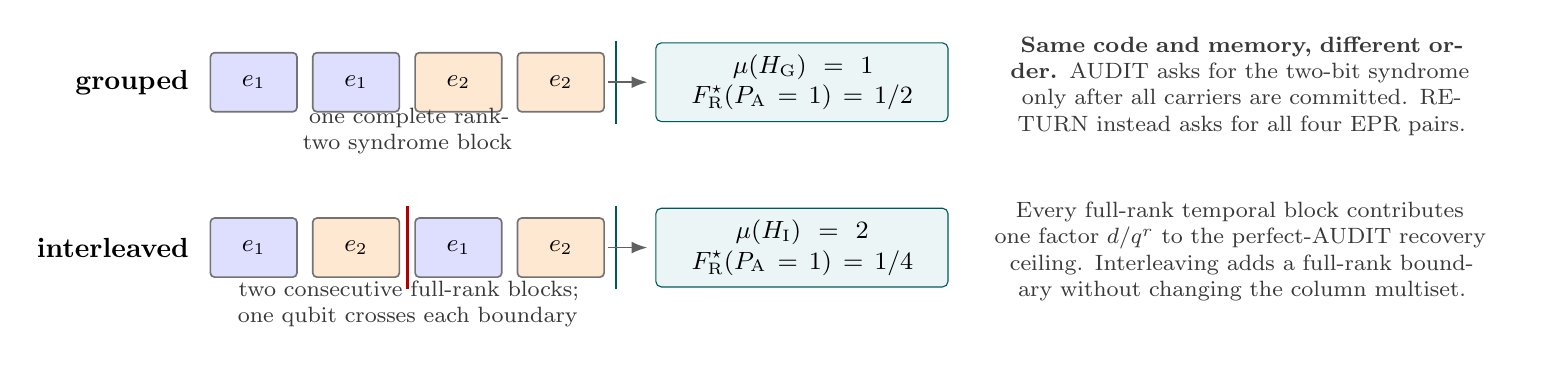
\begin{tikzpicture}[
  x=1cm,y=1cm,font=\small,
  cell/.style={draw=black!55, rounded corners=1.5pt, minimum width=11mm,
    minimum height=7.5mm, line width=0.6pt},
  acol/.style={cell, fill=blue!13},
  bcol/.style={cell, fill=orange!18},
  endpoint/.style={draw=teal!70!black, fill=teal!8, rounded corners=2pt,
    text width=35mm, minimum height=10mm, align=center, inner sep=3pt},
  note/.style={font=\footnotesize, align=center, text=black!78},
  arrow/.style={-{Latex[length=2mm]}, line width=0.65pt, draw=black!62}
]
  \node[font=\bfseries, anchor=east] at (-0.25,1.1) {grouped};
  \node[acol] at (0.45,1.1) {$e_1$};
  \node[acol] at (1.75,1.1) {$e_1$};
  \node[bcol] at (3.05,1.1) {$e_2$};
  \node[bcol] at (4.35,1.1) {$e_2$};
  \draw[teal!70!black, line width=1pt] (5.05,1.63) -- (5.05,0.57);
  \draw[arrow] (4.95,1.1) -- (5.45,1.1);
  \node[endpoint, anchor=west] at (5.55,1.1)
    {$\mu(H_{\rm G})=1$\quad
     $F_{\rm R}^{\star}(P_{\rm A}=1)=1/2$};
  \node[note, text width=50mm] at (2.40,0.48)
    {one complete rank-two syndrome block};

  \node[font=\bfseries, anchor=east] at (-0.25,-1.0) {interleaved};
  \node[acol] at (0.45,-1.0) {$e_1$};
  \node[bcol] at (1.75,-1.0) {$e_2$};
  \node[acol] at (3.05,-1.0) {$e_1$};
  \node[bcol] at (4.35,-1.0) {$e_2$};
  \draw[red!70!black, line width=1pt] (2.40,-0.47) -- (2.40,-1.53);
  \draw[teal!70!black, line width=1pt] (5.05,-0.47) -- (5.05,-1.53);
  \draw[arrow] (4.95,-1.0) -- (5.45,-1.0);
  \node[endpoint, anchor=west] at (5.55,-1.0)
    {$\mu(H_{\rm I})=2$\quad
     $F_{\rm R}^{\star}(P_{\rm A}=1)=1/4$};
  \node[note, text width=53mm] at (2.40,-1.72)
    {two consecutive full-rank blocks; one qubit crosses each boundary};

  \node[note, anchor=west, text width=68mm] at (9.45,1.05)
    {\textbf{Same code and memory, different order.} AUDIT asks for the
     two-bit syndrome only after all carriers are committed. RETURN instead
     asks for all four EPR pairs.};
  \node[note, anchor=west, text width=68mm] at (9.45,-1.05)
    {Every full-rank temporal block contributes one factor $d/q^r$ to the
     perfect-AUDIT recovery ceiling. Interleaving adds a full-rank boundary
     without changing the column multiset.};
\end{tikzpicture}
}
\caption{The same four columns in two temporal orders. The grouped stream has
one complete rank-two block. The interleaved stream has two; a one-qubit bond
must cross both full-rank boundaries. AUDIT sees only the classical transcript
and terminal qubit, whereas RETURN regains all committed carriers.}
\label{fig:orders}
\end{figure*}

\begin{resultbox}
For the interleaved stream, every admissible strategy obeys
$\beta_{H_{\rm I},2}(\lambda)\leq\UI(\lambda)$, and
$\UI(\lambda)<\BG(\lambda)$ whenever $3/7<\lambda<1$. Thus temporal order
changes the achievable information--recovery region in the interior, not only
at perfect AUDIT.
\end{resultbox}

The broad ingredients are established. Quantum combs and process tensors
describe multitime strategies and their internal memories
\cite{chiribella2009networks,pollock2018processes,bisio2012memory}. Bounded
coherent memory has been studied through constrained-separability hierarchies
and autonomous process discrimination \cite{ohst2026memory,zonnios2026bounded}.
Postmeasurement-information games allow unlimited classical data beside a
bounded quantum register \cite{konig2005power,ballester2008postmeasurement},
while information--disturbance theory relates measurement records to later
recovery \cite{banaszek2001fidelity,gregoratti2003lostfound,hsieh2026interactive}.
Classical trellis complexity is famously order dependent
\cite{forney1994trellis,mceliece1996bcjr,kashyap2008pathwidth}. The claim here
is narrower: an exact same-code temporal-order separation in a common-prefix
syndrome-AUDIT/all-carrier-RETURN game, together with a causal-list rank-tail
bound. A focused search through 21 August 2026 located no direct antecedent of
that conjunction; this is a dated collision assessment through 22 August 2026,
not proof of priority.

\section{Late-choice streaming model}
\label{sec:model}

At slot $i\in\{1,\ldots,n\}$, the verifier prepares
\begin{equation}
\ket{\Phi^+}_{R_iA_i}=\frac{\ket{00}+\ket{11}}{\sqrt2},
\end{equation}
sends $A_i$ to the device, receives $B_i$, and immediately sequesters $B_i$.
The device applies an arbitrary adaptive instrument to $A_i$, fresh local
ancillas, and a persistent memory $M_{i-1}$. Only $M_i$, with declared
dimension at most $d_i$, may remain coherent across the next cut. An
unrestricted finite classical transcript is free, but it must be genuinely
dephased: retaining its coherent purification would be an additional quantum
memory.

After slot $n$, a hidden choice selects one task. In AUDIT, the references are
measured in the computational basis, producing a uniform word
$X\in\mathbb F_q^n$. The device receives neither references nor sequestered
carriers and must output the full syndrome $HX\in\mathbb F_q^r$ using only
its transcript and terminal memory. Its unconditional success is $\PA$. In
RETURN, a transcript-conditioned decoder acts jointly on all $B_i$ and the
terminal memory, without reference access. The verifier tests all EPR pairs
and the charged memory reset. Its unconditional acceptance probability is
$\FR$.

For $0\leq\lambda\leq1$, define the support function
\begin{equation}
\beta^{\rm stream}_{H,d}(\lambda)
=\sup_{\mathcal S}\bigl[\lambda\PA(\mathcal S)
+(1-\lambda)\FR(\mathcal S)\bigr],
\label{eq:support}
\end{equation}
where the supremum includes arbitrary finite-outcome adaptive non-QND
strategies satisfying the interface. No postselection is allowed. Immediate
sequestration matters: past carriers cannot silently enlarge a later memory.

For the canonical binary pair,
\begin{equation}
H_{\rm G}=\begin{pmatrix}1&1&0&0\\0&0&1&1\end{pmatrix},\qquad
H_{\rm I}=\begin{pmatrix}1&0&1&0\\0&1&0&1\end{pmatrix}.
\label{eq:matrices}
\end{equation}
They differ only by a coordinate permutation. Both have four equiprobable
syndromes, and the persistent memory is one qubit.

\section{Static ceiling and grouped attainment}
\label{sec:grouped}

Ignoring streaming order gives a useful terminal-dimension relaxation. For a
four-label ensemble and a terminal qubit, the exact support is
\begin{equation}
\BG(\lambda)=
\frac{1+\sqrt{\lambda^2+(1-\lambda)^2}}{2}.
\label{eq:static}
\end{equation}
The bound follows by refining the classical flag, applying the dimension-two
minimum-error bound to AUDIT, and the flagged recovery inequality to RETURN.
For a normalized four-component likelihood row, the extremal profile has two
equal large entries and two equal small entries. The remaining optimization is
the Euclidean norm in \eqref{eq:static}.

\begin{proposition}[Grouped frontier]
For $H_{\rm G}$ and a persistent qubit,
\begin{equation}
\beta^{\rm stream}_{H_{\rm G},2}(\lambda)=\BG(\lambda)
\quad(0\leq\lambda\leq1).
\end{equation}
An exposed parametrization is
\begin{equation}
\PA=\frac{1+t}{2},\qquad
\FR=\frac{1+\sqrt{1-t^2}}2,\qquad0\leq t\leq1.
\label{eq:groupedcurve}
\end{equation}
\end{proposition}

The device coherently accumulates the first parity, weakly records it with
strength $t$, uncomputes the carrier-dependent part, and hands the same qubit
to the second parity. The classical flag and terminal qubit identify the full
syndrome in AUDIT; the carrier outputs undo the coherent updates in RETURN.
At perfect AUDIT, \eqref{eq:groupedcurve} gives $\FR=1/2$.

\section{Temporal fragmentation at perfect audit}
\label{sec:endpoint}

The endpoint extends well beyond the four-slot example. Let
$H\in\mathbb F_q^{r\times n}$ be split into $m$ consecutive blocks,
\begin{equation}
H=[H^{(1)}|\cdots|H^{(m)}],\qquad
\operatorname{rank}H^{(j)}=r.
\label{eq:blocks}
\end{equation}
Put $N=q^r$. Let at most $d_j\leq N$ coherent dimensions cross the boundary
after block $j$, including the terminal boundary. The transcript remains
free and classical.

\begin{theorem}[Perfect-AUDIT temporal product law]
Under \eqref{eq:blocks},
\begin{equation}
\PA=1\quad\Longrightarrow\quad
\FR\leq\prod_{j=1}^{m}\frac{d_j}{N}.
\label{eq:productlaw}
\end{equation}
For uniform $d=q^s$, the bound is attained on
$H=[I_r|\cdots|I_r]$ by retaining $s$ syndrome coordinates coherently and
recording the other $r-s$ coordinates in each block.
\end{theorem}

Each full-rank block introduces an independently uniform syndrome
contribution. Perfect terminal decoding constrains every refined Kraus leaf
to at most $d_j$ cumulative labels at boundary $j$. Intersecting those
constraints leaves a support fraction $\prod_j(d_j/N)$. Optimal flagged
recovery converts that rank fraction into \eqref{eq:productlaw}.

For $H_{\rm G}$, one can pack only one consecutive full-rank block, so the
endpoint is $1/2$. For $H_{\rm I}=[I_2|I_2]$, there are two and the endpoint
is $1/4$. Both are attained. Repeating each basis column $m$ times gives a
larger same-columns separation: batching equal columns yields $d/q^r$, while
cycling through the basis $m$ times yields $(d/q^r)^m$. The ratio grows as
$(q^r/d)^{m-1}$. Consecutive trellis sectionalization itself is classical
prior art \cite{lafourcade1996sectionalization}; the new statement is the
late-choice recovery law attached to it.

\section{Causal lists and a linear spectral tail}
\label{sec:robust}

Perfect decoding forces exact low rank. Approximate decoding requires a
quantitative substitute. Let $D=q^n$ and
\begin{equation}
\alpha=\prod_{j=1}^{m}\frac{d_j}{N},\qquad
k=\alpha D=q^{n-mr}\prod_jd_j.
\label{eq:alphak}
\end{equation}
Refine every instrument outcome to a single Kraus label and reveal the label
to both late decoders. This only enlarges the strategy class. A complete
transcript $c$ has a sequential Kraus operator $K_c$ and effect
$G_c=K_c^\dagger K_c$. Let
\begin{equation}
t_c=\sum_{\ell>k}\lambda_\ell(G_c),
\label{eq:tail}
\end{equation}
where eigenvalues are nonincreasing.

\begin{theorem}[Linear rank-tail robustness]
For every admissible strategy under \eqref{eq:blocks}, with
$\epsilon=1-\PA$,
\begin{equation}
\boxed{\sum_c t_c\leq mD\epsilon.}
\label{eq:lineartail}
\end{equation}
Consequently, for
$\theta=\min\{m\epsilon,1-\alpha\}$,
\begin{equation}
\boxed{
\FR\leq\alpha+(1-2\alpha)\theta
+2\sqrt{\alpha(1-\alpha)\theta(1-\theta)}.}
\label{eq:returnbound}
\end{equation}
\end{theorem}

The proof uses a dimension-to-list conversion. At boundary $j$, pull the
terminal AUDIT measurement backward through the future comb, average over the
independent future inputs, and relabel the final syndrome as the cumulative
prefix syndrome. This produces a valid POVM on the $d_j$-dimensional cut
memory with the same global success $\PA$. A dimension-$d_j$ POVM implies a
classical list $L_j$ of at most $d_j$ labels whose event probability is at
least $\PA$.

For a complete transcript, intersect the $m$ causal list events. Their
failure probability is at most $m\epsilon$. The cumulative block labels are
in bijection with the individual block syndromes, and full rank makes every
fibre uniform. The intersection therefore contains at most $k$ computational
words. Schur--Horn majorisation turns its coordinate mass into the top-$k$
spectral mass of $G_c$, proving \eqref{eq:lineartail}. This route avoids the
extra square-root losses of approximate-injectivity arguments.

To obtain RETURN, split the singular values above and below rank $k$:
\begin{equation}
\Tr\sqrt{G_c}\leq
\sqrt{k(m_c-t_c)}+\sqrt{(D-k)t_c},
\qquad m_c=\Tr G_c.
\label{eq:split}
\end{equation}
Instrument completeness gives $\sum_cm_c=D$. Cauchy--Schwarz sums
\eqref{eq:split}, while Ky Fan anti-norm superadditivity gives the universal
tail ceiling $\sum_ct_c\leq D-k$ \cite{bhatia1997matrix}. Substitution yields
\eqref{eq:returnbound}. The right-hand side is a squared overlap of two real
unit vectors, so its monotonicity on the allowed interval is immediate.

\section{An explicit interior order gap}
\label{sec:gap}

For $H_{\rm I}$, $m=2$ and $\alpha=1/4$. Hence, with
\begin{equation}
\theta=\min\{2(1-\PA),3/4\},
\end{equation}
every strategy satisfies
\begin{equation}
\FR\leq\frac14+\frac12\theta
+\frac{\sqrt3}{2}\sqrt{\theta(1-\theta)}.
\label{eq:interleavedreturn}
\end{equation}
Near perfect AUDIT this becomes
\begin{equation}
\FR\leq\frac14+(1-\PA)
+\sqrt{\frac32(1-\PA)(2\PA-1)}.
\end{equation}
The square-root exponent is optimal: a legal weak-record family has a
$\sqrt{1-\PA}$ correction. The leading constant is not claimed sharp.

Maximizing \eqref{eq:interleavedreturn} in the support direction gives a
closed certificate.

\begin{corollary}[Certified interior separation]
For every $0\leq\lambda\leq1$,
\begin{equation}
\beta^{\rm stream}_{H_{\rm I},2}(\lambda)
\leq\UI(\lambda)
=\frac12+\frac\lambda4
+\frac14\sqrt{7\lambda^2-10\lambda+4}.
\label{eq:UI}
\end{equation}
Moreover,
\begin{equation}
\UI(\lambda)<\BG(\lambda)
\quad\text{for}\quad \frac37<\lambda<1.
\label{eq:strictgap}
\end{equation}
\end{corollary}

Set $\theta=\sin^2\phi$, $0\leq\phi\leq\pi/3$. The support becomes a positive
$2\times2$ quadratic form in $(\cos\phi,\sin\phi)$; its largest eigenvalue is
\eqref{eq:UI}. Eliminating the two radicals when comparing \eqref{eq:UI} with
\eqref{eq:static} gives
$-4\lambda^2(\lambda-1)(7\lambda-3)$, with the unsquared signs fixing the
interval in \eqref{eq:strictgap}.

At balanced weight,
\begin{equation}
\beta^{\rm stream}_{H_{\rm I},2}(1/2)
\leq\frac58+\frac{\sqrt3}{8}
=0.841506350946\ldots,
\end{equation}
whereas the grouped value is
$\BG(1/2)=0.853553390593\ldots$. This proves an interior gap without assuming
QND, Clifford, projective, covariant, or binary-outcome instruments.

\begin{figure*}[t]
\centering
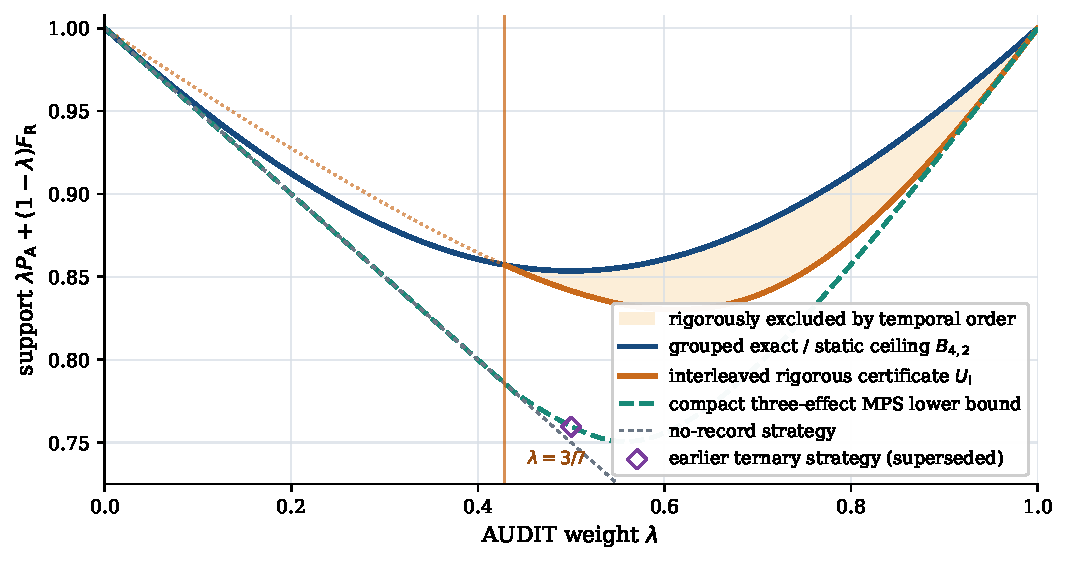
\includegraphics[width=0.94\textwidth]{order_support_gap.pdf}
\caption{Support values for the same-code pair. The blue curve is the exact
grouped frontier. The orange curve is the rigorous interleaved upper
certificate; the shaded region is excluded solely by temporal order for
$3/7<\lambda<1$. The dashed curve is the compact three-effect MPS lower
bound; the hollow diamond is the earlier ternary strategy that it supersedes.
The unclosed vertical distance is not an error bar: it is the remaining
global MPS-maximisation problem.}
\label{fig:support}
\end{figure*}

\section{Exact leaf reduction and compact construction}
\label{sec:numerics}

Write a fine transcript leaf as
$K:A_1\cdots A_4\to B_1\cdots B_4M$. Its vectorisation is an open-boundary
MPS whose three temporal bond ranks are at most two. For a normalised leaf,
define
\begin{align}
A_H(K)&=\max_{\{E_s\}}\sum_x\Tr\!\left[
E_{Hx}\Tr_{B^4}K\proj{x}K^\dagger\right],\label{eq:leafA}\\
R(K)&=\frac1{16}\left(\Tr\sqrt{K^\dagger K}\right)^2,
\qquad \Tr K^\dagger K=1.\label{eq:leafR}
\end{align}

\begin{theorem}[Homogeneous Choi-MPS reduction]
For the interleaved game,
\begin{equation}
\begin{aligned}
\beta^{\rm stream}_{H_{\rm I},2}(\lambda)
&=
\max_{\substack{\Tr K^\dagger K=1\\
\operatorname{TT-rank}_i(\lvert K\rangle\!\rangle)\leq2}}\\[-1mm]
&\quad\left[\lambda A_{H_{\rm I}}(K)+(1-\lambda)R(K)\right].
\end{aligned}
\label{eq:mpsreduction}
\end{equation}
Four classical outcomes per slot suffice.
\end{theorem}

The upper direction is a homogeneous averaging argument: every complete
strategy is a probability distribution over its normalised fine leaves, and
both branch scores average with the same leaf weights. For the converse, put
an arbitrary feasible leaf in row-isometric MPS gauge, with local tensors
$T_i$ satisfying
\begin{equation}
\Tr_{A_i}(T_i^\dagger T_i)=\id_{M_{i-1}}.
\end{equation}
For each Pauli $P\in\{I,X,Y,Z\}$ use the local Kraus map
$T_i(P\otimes\id)/\sqrt2$. The Pauli one-design identity makes these four
maps complete. Every four-slot transcript is $K$ right-multiplied by a tensor
product of Paulis and scaled by $1/4$. RETURN is invariant, while the known
Pauli bit flips merely relabel the linear syndrome in AUDIT. Thus all 256
leaves have the same homogeneous score, proving \eqref{eq:mpsreduction}.

The strongest compact construction found inside \eqref{eq:mpsreduction} has
three nonzero rank-one effects. It admits a two-variable support formula. Put
\begin{align}
g&=1-t/2,& z&=-t/(2-t),\notag\\
e&=t(1+r)/2,\notag\\[-1mm]
\Delta&=\sqrt{(1-z^2)(1-r^2)},\notag\\[-1mm]
h&=\frac g2(1+zr+\Delta),\label{eq:compacth}\\
c_0&=\sqrt t+\sqrt{1-t},&
c_1&=\sqrt e+\sqrt{1-e},\notag
\end{align}
and let $c_\varnothing=\sqrt2$ for $t\geq1/2$, while
$c_\varnothing=c_0$ for $t<1/2$. Define
\begin{equation}
\begin{aligned}
\bm c&=(c_0,c_\varnothing,\sqrt2c_1)^{\mathsf T},\\
M_\lambda(t,r)&=\lambda\operatorname{diag}(t,0,h)
+\frac{1-\lambda}{8}\bm c\bm c^{\mathsf T}.
\end{aligned}
\label{eq:compactmatrix}
\end{equation}
Then the physical lower bound is
\begin{equation}
L_{\rm I}(\lambda)=\max\left\{1-\frac\lambda2,
\max_{\substack{0\leq t\leq1\\-1\leq r\leq1}}
\lambda_{\max}\bigl(M_\lambda(t,r)\bigr)\right\}.
\label{eq:compactlower}
\end{equation}
The Perron eigenvector fixes the four middle-cut priors. The first two slots
prepare those four pure states; slot three implements the three-effect POVM;
slot four generates a uniform bit and XORs the binary decision into the
terminal qubit. Orthogonal emitted states make $K^\dagger K$ diagonal, so the
polar RETURN value in \eqref{eq:leafR} is attained exactly.

At balanced weight, \eqref{eq:compactlower} gives
\begin{align}
t&=0.458073977\ldots,\notag\\
r&=0.016373524\ldots,\notag\\
\PA&=0.620085075586\ldots,\notag\\
\FR&=0.899520492117\ldots,\notag\\
L_{\rm I}(1/2)&=0.759802783851444\ldots .
\label{eq:balancedcompact}
\end{align}
It crosses the no-record line at
$\lambda_c=0.441437845098\ldots$. An independent NumPy construction checks
all temporal ranks, local row isometries, Pauli completeness, and direct
scores; its largest residual is below $9\times10^{-16}$.

Unrestricted complex Choi-MPS continuation, eight multistarts of the larger
pinched cq-instrument relaxation, and a relaxation of the first two slots all
agree with \eqref{eq:compactlower} on the tested grid. This is substantially
stronger evidence than the earlier ternary tree value
$0.759448970317\ldots$, and Pauli completion proves that the compact leaf is
itself physical. It is still not a global upper certificate for
the nonconvex maximum in \eqref{eq:mpsreduction}; equality between
$L_{\rm I}$ and the exact support remains a conjecture.

\section{Relation to neighbouring disciplines}

The result sits at a specific intersection. Bounded-storage cryptography and
postmeasurement information already turn a quantum dimension into a late
decoding limitation \cite{konig2005power,ballester2008postmeasurement}.
Quantum-comb memory cost already separates persistent coherent dimensions
from classical assistance \cite{bisio2012memory,ohst2026memory}. Sequential
state generation identifies persistent ancilla dimension with a temporal
tensor-network bond \cite{li2022emitters}. Trellises, sectionalization, and
matroid pathwidth already quantify order-sensitive live constraints in linear
codes \cite{forney1994trellis,lafourcade1996sectionalization,kashyap2008pathwidth}.
Nondestructive discrimination connects classical labels with recoverable
entanglement in a spatial LOCC setting \cite{bilash2024nondestructive,lim2025local}.

The present bridge is operational rather than terminological. A causal
dimension bound is converted into one classical list at every full-rank
temporal section. The intersection size controls a Ky Fan tail of each
instrument leaf, which in turn controls all-carrier entanglement recovery.
None of the nearby papers located in the focused review states this chain for
the same-code, late-choice syndrome/return interface. Conversely, the work
does not claim that order dependence, trellis width, bounded quantum memory,
or information--disturbance is new in isolation.

\section{Limits and open exact frontier}

The theorem is conditional on a trusted resource boundary. Every coherent
system crossing a block cut must count toward $d_j$; the classical transcript
must be dephased; past carriers must be unavailable in AUDIT; and RETURN must
include all failures. Relaxing any of these assumptions changes the task.
Visible memory reset does not prove that an inaccessible environment contains
no record.

The interval \eqref{eq:strictgap} resolves the existence of an interior order
effect, not the full interleaved Pareto boundary. At balanced weight the best
verified lower strategy and rigorous upper certificate are
\begin{align}
0.759802783851\ldots
&\leq\beta^{\rm stream}_{H_{\rm I},2}(1/2)\notag\\[-1mm]
&\leq0.841506350946\ldots.
\end{align}
The Choi-MPS reduction proves that local completeness and unbounded adaptive
outcome trees are no longer the obstruction. Closing the gap now requires
either a better bond-two MPS leaf or a global upper certificate for the
nonconvex quotient in \eqref{eq:mpsreduction}. The optimal coefficient in the
near-endpoint square-root law and extensions to partially ranked block
sequences are also open.

Nothing in the observed statistics selects an interpretation of quantum
mechanics. The result is a standard operational statement about coherent
memory, temporal order, and recoverability. It neither observes alternative
worlds nor communicates with an environmentally decohered branch.

\section{Conclusion}

Permuting the columns of one linear syndrome can change the attainable
information--recovery region of a fixed coherent memory. Grouping equal
columns allows a one-qubit device to attain the static frontier; interleaving
them creates an additional full-rank temporal boundary, squares the
perfect-AUDIT recovery penalty, and produces a rigorously certified interior
gap. Causal list decoding provides the robust mechanism: approximate terminal
knowledge yields small lists at every memory cut, their intersection bounds a
spectral tail, and that tail limits coherent recovery. This narrow theorem,
rather than a many-worlds narrative, is the contribution that survives the
originality audit. Local Pauli completion further removes the arbitrary
adaptive tree exactly and leaves one finite bond-two Choi-MPS maximum. The
three-effect construction gives the strongest verified lower curve, but the
remaining global maximum is deliberately left open.

\appendix
\section{Dimension-to-list lemma}
\label{app:list}

\begin{lemma}
Let $\{\rho_x\}_{x\in\mathcal X}$ be subnormalised states on a
$d$-dimensional system and $\{E_x\}_{x\in\mathcal X}$ a POVM. If
$p_x=\Tr\rho_x$, then
\begin{equation}
\sum_x\Tr(E_x\rho_x)
\leq\max_{L\subseteq\mathcal X,\,|L|\leq d}\sum_{x\in L}p_x.
\label{eq:listlemma}
\end{equation}
\end{lemma}

\begin{proof}
Positivity gives
$\Tr(E_x\rho_x)\leq p_x\lVert E_x\rVert_\infty$. The weights
$w_x=\lVert E_x\rVert_\infty$ satisfy $0\leq w_x\leq1$ and
\begin{equation}
\sum_xw_x\leq\sum_x\Tr E_x=d.
\end{equation}
The resulting fractional $d$-unit linear program assigns unit weight to the
$d$ largest $p_x$, proving \eqref{eq:listlemma}.
\end{proof}

\section{Pulled-back boundary measurements}
\label{app:pullback}

Write a word as blocks $x=(x_1,\ldots,x_m)$ and define
\begin{equation}
v_j=H^{(j)}x_j,\qquad u_j=v_1+\cdots+v_j.
\end{equation}
Let $a_j$ be the refined transcript through boundary $j$. Conditioned on
$a_j$ and $u_j=u$, trace all sequestered prefix carriers and within-fibre
variables, producing a subnormalised state $\rho^{(j)}_{a_j,u}$ on the cut
memory.

Fix the future block inputs and compose the suffix comb with the terminal
AUDIT POVM. Relabel its final answer $u_m$ as
\begin{equation}
u_j=u_m-(v_{j+1}+\cdots+v_m).
\end{equation}
Averaging these effects over independent uniform future inputs gives a POVM
on the cut memory. Summed over prefix transcripts, its success is the original
$\PA$. The construction remains valid when the cut memory is entangled with
past carriers: the future comb acts only on the memory and the carriers are
traced in AUDIT.

Applying \cref{app:list} at every prefix transcript gives a classical list
$L_j(a_j)\subseteq\mathbb F_q^r$, $|L_j(a_j)|\leq d_j$, such that
\begin{equation}
\Pr[U_j\in L_j(A_j)]\geq\PA.
\label{eq:listevent}
\end{equation}
The POVMs for different $j$ need not be jointly measurable; the lists are
proof objects, not simultaneous physical measurements.

For a complete transcript $c$, define
\begin{equation}
S_c=\{x:u_j(x)\in L_j(a_j(c))\text{ for all }j\}.
\end{equation}
The map $(u_1,\ldots,u_m)\leftrightarrow(v_1,\ldots,v_m)$ is bijective.
Every full-rank block has fibre size $q^{n_j-r}$, hence
\begin{equation}
|S_c|\leq q^{n-mr}\prod_jd_j=k.
\end{equation}
The union bound applied to \eqref{eq:listevent} yields
\begin{equation}
\sum_c\sum_{x\notin S_c}\lVert K_c\ket{x}\rVert^2
\leq mD(1-\PA).
\label{eq:coordinateoutside}
\end{equation}
The diagonal of $G_c$ is precisely
$\lVert K_c\ket{x}\rVert^2$. Schur--Horn majorisation implies that the
diagonal mass on any set of at most $k$ coordinates is no greater than the
sum of the top $k$ eigenvalues. Subtracting from $\Tr G_c$ in
\eqref{eq:coordinateoutside} proves \eqref{eq:lineartail}.

\section{From spectral tail to recovery}
\label{app:recovery}

For a fine-grained leaf, optimal polar correction contributes at most
\begin{equation}
F_{{\rm R},c}\leq\frac{(\Tr\sqrt{G_c})^2}{D^2}.
\label{eq:polar}
\end{equation}
This already allows a joint decoder on every emitted carrier and terminal
memory; dropping the reset projector is an upper relaxation. Applying
Cauchy--Schwarz separately to the first $k$ and last $D-k$ singular values
gives \eqref{eq:split}. Let $T=\sum_ct_c=\theta'D$. Since
$\sum_cG_c=\id_D$, one has $\sum_cm_c=D$. Summing the square of
\eqref{eq:split} and applying Cauchy--Schwarz to
$\sum_c\sqrt{t_c(m_c-t_c)}$ gives
\begin{equation}
\FR\leq\alpha+(1-2\alpha)\theta'
+2\sqrt{\alpha(1-\alpha)\theta'(1-\theta')}.
\end{equation}
The sum of the smallest $D-k$ eigenvalues is a homogeneous concave spectral
functional, hence superadditive. Therefore
\begin{equation}
T\leq\sum_{\ell>k}\lambda_\ell\!\left(\sum_cG_c\right)=D-k.
\end{equation}
Together with \eqref{eq:lineartail}, this gives
$0\leq\theta'\leq\min\{m(1-\PA),1-\alpha\}$. The recovery expression is
increasing throughout that interval, proving \eqref{eq:returnbound}.

\section{Homogeneous Choi-MPS completion}
\label{app:paulicompletion}

This appendix proves \eqref{eq:mpsreduction}. Refine every classical
transcript of a physical four-slot strategy until it has one global Kraus
operator $K_c$, and put
\begin{equation}
G_c=K_c^\dagger K_c,\qquad t_c=\Tr G_c.
\end{equation}
Instrument completeness gives $\sum_cG_c=\id_{16}$ and
$\sum_ct_c=16$. For $t_c>0$, write
$\widehat K_c=K_c/\sqrt{t_c}$. Because the terminal measurement and flagged
recovery may depend on $c$, the two branch scores decompose exactly as
\begin{equation}
\PA=\sum_c\frac{t_c}{16}A_{H_{\rm I}}(\widehat K_c),
\qquad
\FR=\sum_c\frac{t_c}{16}R(\widehat K_c).
\label{eq:leafaverage}
\end{equation}
The weights in \eqref{eq:leafaverage} sum to one. Every leaf has temporal TT
ranks at most two, so its support score is no larger than the right-hand side
of \eqref{eq:mpsreduction}. This proves the upper direction independently of
the number or adaptivity of the outcomes.

For the converse, take any normalised operator $K$ admitted by the maximum in
\eqref{eq:mpsreduction}. Successive Schmidt decompositions put its
vectorisation in row-isometric MPS gauge. Its local tensors
\begin{equation}
T_i:A_i\otimes M_{i-1}\longrightarrow B_i\otimes M_i
\end{equation}
obey
\begin{equation}
\Tr_{A_i}(T_i^\dagger T_i)=\id_{M_{i-1}}.
\label{eq:rowgauge}
\end{equation}
Zero Schmidt subspaces may be removed and smaller bonds padded, so this gauge
does not increase the allowed memory dimension.

For $P\in\{I,X,Y,Z\}$, define the four local Kraus maps
\begin{equation}
L_{i,P}=2^{-1/2}T_i(P\otimes\id_{M_{i-1}}).
\label{eq:localkraus}
\end{equation}
The Pauli one-design identity
\begin{equation}
\sum_P(P^\dagger\otimes\id)Y(P\otimes\id)
=2\id_{A_i}\otimes\Tr_{A_i}Y
\end{equation}
together with \eqref{eq:rowgauge} yields
$\sum_PL_{i,P}^\dagger L_{i,P}=\id_{A_iM_{i-1}}$. Thus
\eqref{eq:localkraus} is a complete causal instrument at every slot and its
outcome may be dephased immediately.

For a full Pauli transcript ${\bm P}=(P_1,\ldots,P_4)$, contraction gives
\begin{equation}
K_{\bm P}=\frac14K(P_1\otimes\cdots\otimes P_4).
\label{eq:covariantleaves}
\end{equation}
All 256 leaves have $
\Tr K_{\bm P}^\dagger K_{\bm P}=1/16$ and hence probability $1/256$ on
the maximally mixed input. Right-unitary invariance preserves $R(K)$. If
$P_i=X^{a_i}Z^{b_i}$, then $P_i\ket{x_i}$ is a phase times
$\ket{x_i+a_i}$; subtracting the known shift
$H_{\rm I}(a_1,\ldots,a_4)$ from the terminal answer preserves $A_{H_{\rm
I}}(K)$. Every conditional leaf therefore has the same two scores as $K$.
Their complete mixture attains its homogeneous quotient and proves the lower
direction of \eqref{eq:mpsreduction}.

\section{Reproducibility and claim boundary}

The code, stored instrument, tests, literature ledger, and both manuscript
sources are public at \url{https://github.com/asim-v/carmenq}. The commands
\begin{quote}\ttfamily\scriptsize
python -m pytest -q\\
python scripts/verify\_interleaved\_counterexample.py\\
python scripts/verify\_compact\_interleaved\_candidate.py\\
python scripts/generate\_order\_gap\_figure.py\\
python scripts/build\_order\_pdf.py
\end{quote}
reproduce the software checks, both balanced constructions, plotted bounds,
and this PDF. Numerical searches are explicitly lower-bound generators. The
proved claims are \eqref{eq:productlaw}, \eqref{eq:lineartail},
\eqref{eq:returnbound}, \eqref{eq:mpsreduction}, the attainability of
\eqref{eq:compactlower}, and the interval \eqref{eq:strictgap}. Equality
between \eqref{eq:compactlower} and the exact interleaved interior curve is
not claimed.

\FloatBarrier
\bibliographystyle{unsrt}
{\small\bibliography{../references/library}}

\end{document}
